\tikzset{every picture/.style={line width=0.75pt}} %set default line width to 0.75pt        

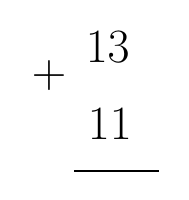
\begin{tikzpicture}[x=0.75pt,y=0.75pt,yscale=-1,xscale=1]
%uncomment if require: \path (0,300); %set diagram left start at 0, and has height of 300

%Straight Lines [id:da811664255606055] 
\draw    (325,90.6) -- (366,90.6) ;

% Text Node
\draw (329,22) node [anchor=north west][inner sep=0.75pt]  [font=\LARGE] [align=left] {13};
% Text Node
\draw (330,59) node [anchor=north west][inner sep=0.75pt]  [font=\LARGE] [align=left] {11};
% Text Node
\draw (303,36) node [anchor=north west][inner sep=0.75pt]  [font=\LARGE] [align=left] {+};


\end{tikzpicture}